\section{Function}

Function, obviously, is often very difficult to ascertain. For this reason some
studies explicitly ignore orphans altogether \cite{krehenwinkel_eco-genomic_2015}.

\subsection{Expression patterns}

   There is a lot more I could write on this. 

\subsection{Stress/ecological conditions}
   Increase in expression of lineage-specific genes in Daphnia
   \cite{voolstra_rapid_2011}

   So pretty much everything is related to stress. 832/1007 POFs all
   related to at least one measure of abiotic stress
   \cite{luhua_linking_2013}.

   Just because something is upregulated with stress, does not mean it is
   actually functionally related to stress response. A study of fungal four
   orphans in a rust fungi examplify this \cite{sadat_analysis_2014}.

   Two Brassicacea-specific genes in Arabidopsis (ASR35 and ASR63) were
   identified that conferred tolerance to salt stress and iron deficiency,
   respectively \cite{swamidatta_functional_2015}. 

\subsection{Fungal effectors}

    \subsubsection{Paper overview}

    Stergiopoulos et al. (2009) \cite{stergiopoulos_fungal_2009} wrote a very
    large review on the  topic. ``It is accepted that most fungal avirulence
    genes encode virulence factors that are called effectors. Most fungal
    effectors are secreted, cysteine-rich proteins''.

    Here is a great review \cite{de_jonge_how_2011}

    \subsubsection{Terms}

    \begin{description}
        \item[Gene-for-gene hypothesis] One host R gene for each pathogen
            avirulence gene. Effectors are agents that suppress the host immune
            response.
        \item[Pathogen-Associated Molecular Pattern (PAMP)] Regonizable
            features of pathogens used be host in specific defense (for
            example, chitin).
        \item[Effector] Pathogen secreted virulence factors (including small
            cystein-rich proteins). Most effectors are short and have little
            extra-species homology \cite{stergiopoulos_fungal_2009,
            bowen_venturia_2011}.
        \item[Small cystein-rich proteins] A subset of effectors. As their name
            suggests, they are defined as being short (<xxx) and rich in
            cystein (xxx).     
    \end{description}

    \subsubsection{Ideas}

    Most effectors are short and have little extra-species homology
    \cite{stergiopoulos_fungal_2009, bowen_venturia_2011}. Whether they are
    de novo orphans or simply very fast evolvers is an interesting
    question. 

    Most fungal effectors are species-specific based on \textit{Blumeria
    graminis} genome and two relatives (with 70 million years to MRCA)
    \cite{spanu_genome_2010}. Only about 10/248 had homologs in one of the
    nearest two relatives (tBLASTn e-5). 79\% are over-represented in
    haustorium (parasitic hypha that thread between plant cells). They are
    extremely diverse with few members grouping into families. 80\% share an
    N-terminal 'YxC' motif. (see Spanu genome project entry)

    Fungal effectors are so prone to being species-specific that the discover
    of orthologs is noteworthy \cite{bolton_novel_2008,
    stergiopoulos_tomato_2010}. 8 effectors had previously been characterized
    and none had orthologs, Bolton discovered three new ones, one (Ecp6) of which had
    a detectable homolog \cite{bolton_novel_2008}.

    Wulff review argues for extreme specificity of fungal effectors
    \cite{wulff_recognitional_2009}.
    
    Stergipoulos challenges Wulff on the point of host-sepcificity, arguing
    that there is an underlying homology, a core set of effectors that diverges
    into many roles, that can work beyond the limited plant-specific capacity
    \cite{stergiopoulos_tomato_2010}. He doesn't contest the prevalence of
    species-specificity, but offers two new counter examples (Avr4 and Ecp2).

    There are some very large families (e.g. RXLR and Crinkle (CRN)) of
    effectors that are believed to multiply by gene duplication and then
    diversify beyond recognition \cite{haas_genome_2009}.

    \subsubsection{Specific effectors}

    \begin{description}

        \item[Avr line] cloned from \textit{Cladosporium
            fulvum}. A few have homologs.

        \begin{description}
            \item[Avr2] length: 78(58). Inhibits at least 4 cycteine proteases
                (74, 102, 107 refs from paper
                \cite{stergiopoulos_fungal_2009}).
            \item[Avr4] length: 135(86). protects against chitinases
            \item[Avr4E] length: 121(101). 
            \item[Avr9]  length: 63(28).
        \end{description}

        \item[Ecp line] Extracellular Proteins (Ecp) cloned from
            \textit{Cladosporium fulvum} (Ecp1, Ecp2, Ecp4, Ecp5, Ecp6, and
            Ecp7). Only Exp6 has homologs to proteins in other databases
            \cite{stergiopoulos_fungal_2009}. Ecp6 has a LysM domain.

        \item[\textit{Fusarium oxysporum} effectors]

    \end{description}


\subsection{Toxins and defensins}

14 of 20 nematocyte toxins (proteins identified by mass spectroscopy) appear to
be cnidarian-specific (interestingly several of these proteins are small
cystein rich secretory proteins, like many of the fungal effectors, apparently
these are pretty common in toxins) \cite{moran_analysis_2012}.

CRISP proteins comprise $4.3\%$ of Bothriechis supraciliaris pitviper toxins
\cite{lomonte_snake_2012}. CRISPS are NOT all orphans, some are widely
conserved, also the word is used differently in defferent areas
\cite{yamazaki_wide_2003}. Specifically, the fungal effector people add
shortness to the criteria, other people don't. The CRISP and CAP families of
C-rich secretory proteins are indeed often conserved, strike this from the list
\cite{schreiber_novel_1997}.

Plant defensins are also CRISP. But they are not necessarily orphans
\cite{rogozhin_novel_2011}. Some studies of plant reaction to pathogens
specifically ignore orphans \cite{portillo_distinct_2013}

\subsection{Symbiotic communication}

    Aphid bacteriocytes, aphid-specific cell types specialized for cultivating the
    bacterial symbiont Buchnera aphidicola, are enriched in small, species-specific,
    cysteine rich secretory signal proteins \cite{shigenobu_aphids_2012}.

    7-38\% of the genes induced under symbiotic conditions in a large family of
    fungi are orphans \cite{kohler_convergent_2015}.

    \begin{quote}
        The ECM lifestyle in \emph{Laccaria bicolor} is associated with the expression of
         new mycorrhiza- induced small secreted proteins that are required for
         establishment of symbiosis.
     \end{quote}

     ECM mean ectomycorrhizal

\subsection{Species-specific structures}

    Orphan genes may be enriched in lineage-specific structures. A stunning
    example of this comes from the cnidarian phylum, which includes jellyfish
    and Sea anemones. A unique feature of the cnidarian phylum is the
    sting-cell, or nematocyte. These cells, when stimulated, can hurl threads
    (from organelles, called nematocysts) which can act as potentially
    poisonous harpoons, grapples to draw in prey, or tethers to attach to
    surfaces \cite{kass-simon_behavioral_2002}.

    Fish antifreeze protein, \cite{chen_evolution_1997}.

    \begin{figure}[h!]
        \centering
        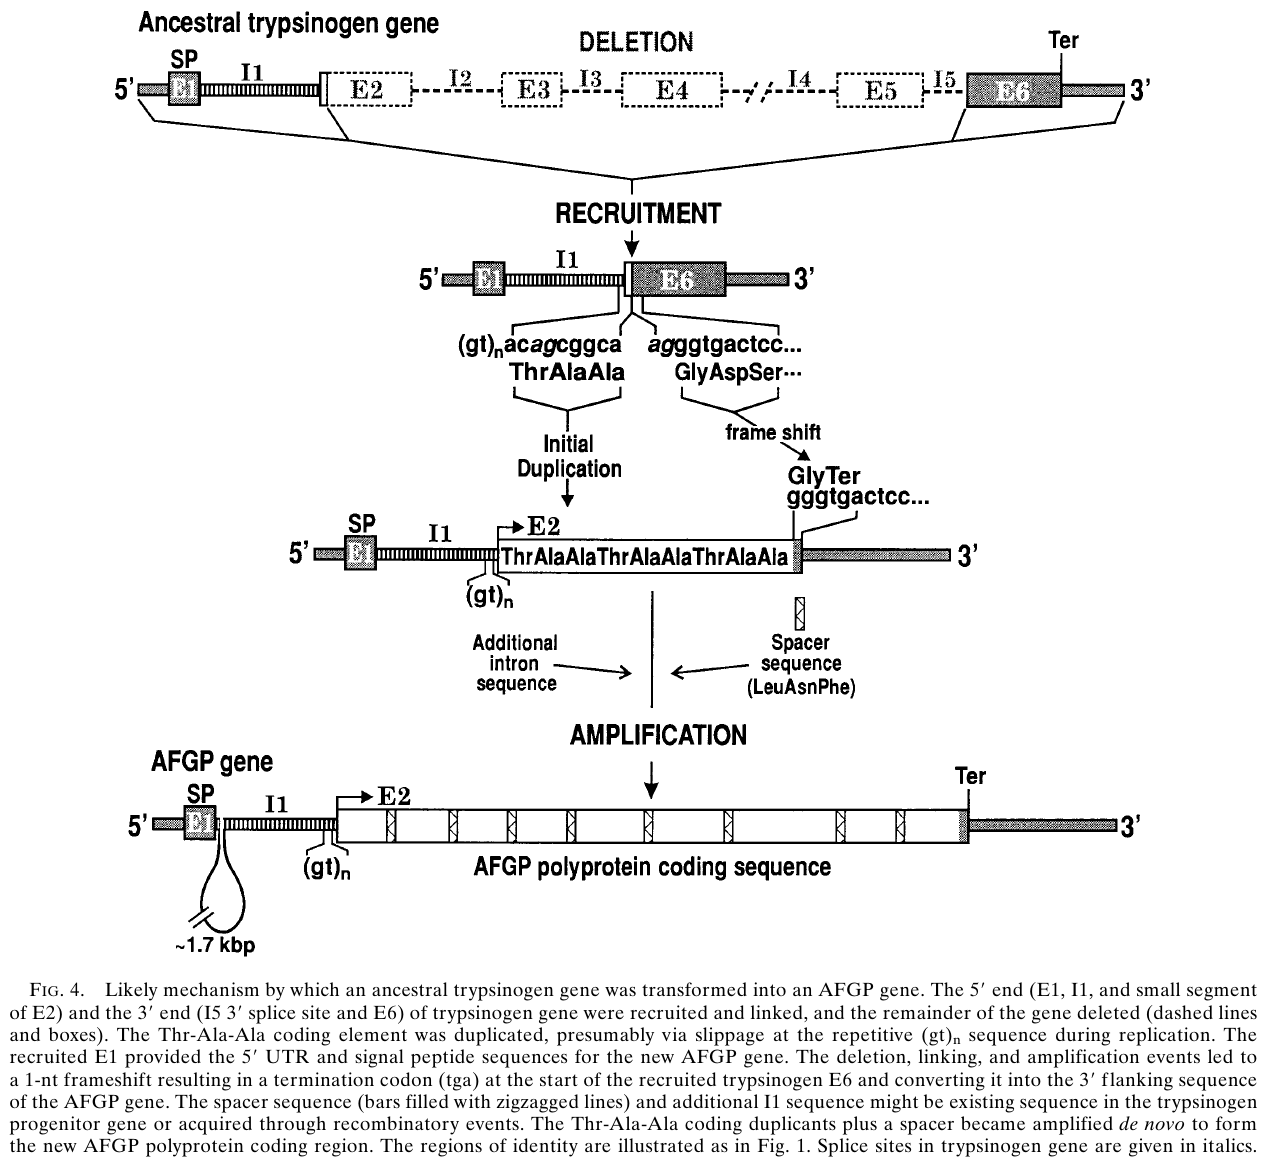
\includegraphics[width=0.8\textwidth]{chen-antifreeze-1997-fig4}
        \caption{Chen (1997) \cite{chen_evolution_1997}}
    \end{figure}
    \FloatBarrier

\subsection{Parasitism/pathogenesis}

  Strong circumstantial evidence that orphans of \textit{Leishmania major} are
  involved in pathogensis \cite{mukherjee_elucidating_2015}.

\subsection{Young genes are seldom catalytic}

    They are NOT recruited as catalysts in secondary metabolism. If there were
    an catalytic arena in which you would expect orphans to be present, it
    would be this, but they are not there (see next section)

\subsection{Regulators of Secondary Metabolism?}

\subsubsection{Specialized enzymes have low specificity}

    The enzymes of secondary metabolism, specialized enzymes, are ~30 times
    less specific than core enzymes \cite{bar-even_moderately_2011}.

\subsubsection{Generally originate via duplication}

    They usually are the promiscuous cousins of core enzymes. By reducing
    specificity, caused by a decrease in order resulting from mutational
    degredation, they are freed to explore new space \cite[review]{weng_rise_2012}.

\subsubsection{Deep evolutionary story}

    Weng story \cite{weng_rise_2012}: The earliest enzymes were very random,
    non-robust, non-specific, and low efficiency. They gradually improved,
    learning to catalyze the core pathways with great efficiency. Secondary
    metabolism followed as duplicates of these ancient enzymes regressed to
    less ordered, more promiscuous, states and explored new pathways.

\subsubsection{Enzymes poorly conserved}

    In 18 Dothideomycetes (fungi) genomes, secondary enzymes show extreme
    diversity \cite{ohm_diverse_2012}.

    Species-sepcific genes twice as common among small secreted proteins
    \cite{ohm_diverse_2012}. 

\subsection{Plant specific features}

    Trichomes

    Secondary metabolites

    Transposon sea

    Synteny and colinearity (2008, but heavily cited, breadcrumbs)
    \cite{tang_synteny_2008}.

\subsection{Development}

  This paper on the development of muscle tissue discusses the general role of
  orphans in developmental cascades \cite{andrikou_too_2015}:

  \begin{quote}
    The integration of species-specific or orphan genes within developmental
    regulatory cascades is another means of evolutionary divergence and is
    repeatedly seen in the animal kingdom. For instance, in sea urchins, a
    species specific Fox gene, FoxY, is upstream of the myogenic network. In
    ascidians a key myogenic factor that plays an important role in the primary
    muscle cell lineage specification, Macho-1, is a specific maternal factor of
    that phylum. Also, in C.elegans, a unique transcription factor, FOZI-1,
    functions in the M lineage for the proper myoblast specification of body wall
    muscles. Moreover, Him a Drosophilid specific gene is necessary for proper
    muscle differentiation.
  \end{quote}
